\documentclass{article}
\usepackage[utf8]{inputenc}

\title{CS246 Homework 3 Answers}
\author{Charlie Zhang}
\date{Feb 2013}

\usepackage{natbib}
\usepackage{float}
\usepackage{graphicx}
 \usepackage{indentfirst}
\usepackage{mathtools}
\usepackage{setspace}
\linespread{1.8}

\begin{document}

\maketitle
\section{Question 1 -- Latent Features for Recommendations}


\subsection{(a)}
$\epsilon_{iu} = r_{iu} - q_i * p_u^T$

$q_i \leftarrow q_i + \eta(\epsilon_{iu}p_u - \lambda q_i)$

$p_u \leftarrow p_u + \eta(\epsilon_{iu}q_i - \lambda p_u)$

Where $\eta$ is the learning rate.

\subsection{(b)}
\begin{figure}[H]
\centering
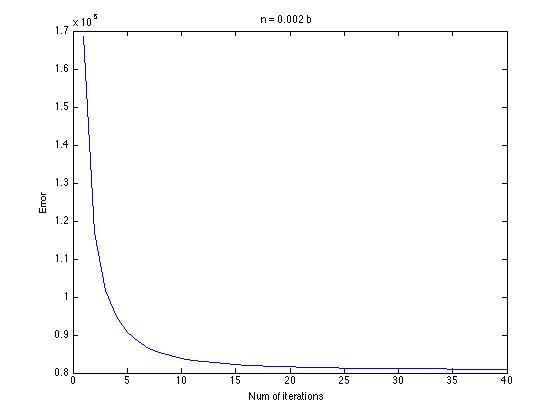
\includegraphics[scale=0.5]{EAsOfIterationEta0002.jpg}
\caption{ Error in first 40 iterations with $\eta=0.002$: }
\label{}
\end{figure}


\subsection{(c)}
\begin{figure}[H]
\centering
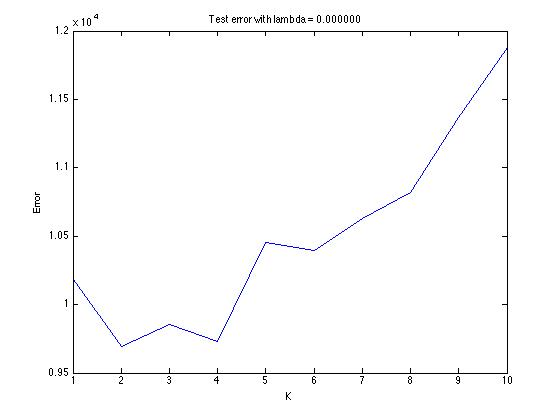
\includegraphics[scale=0.5]{TestErrorLambda0.jpg}
\caption{ $E_{te}$ as of K with $\lambda=0.0$:}
\label{}
\end{figure}

\begin{figure}[H]
\centering
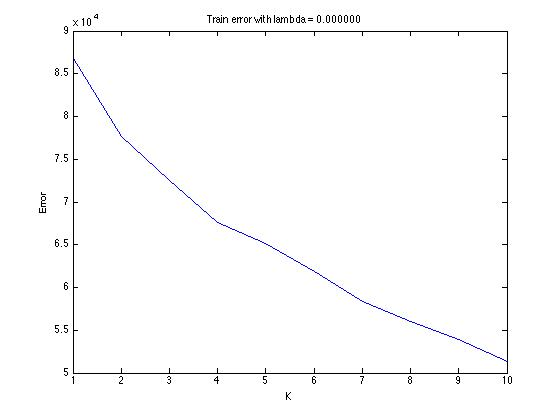
\includegraphics[scale=0.5]{TrainErrorLambda0.jpg}
\caption{ $E_{tr}$ as of K with $\lambda=0.0$:}
\label{}
\end{figure}

\begin{figure}[H]
\centering
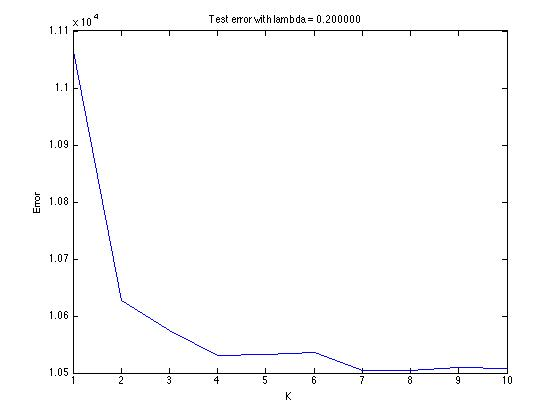
\includegraphics[scale=0.5]{TestErrorLambda02.jpg}
\caption{ $E_{te}$ as of K with $\lambda=0.2$:}
\label{}
\end{figure}

\begin{figure}[H]
\centering
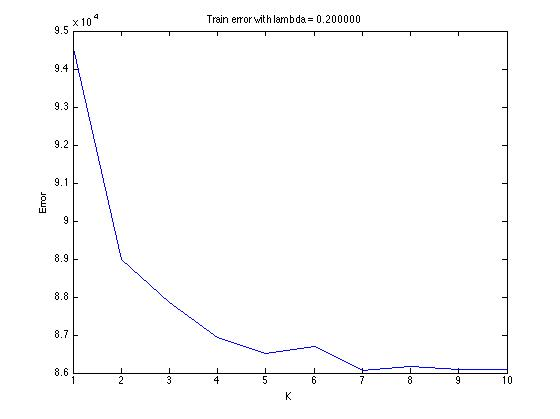
\includegraphics[scale=0.5]{TrainErrorLambda02.jpg}
\caption{ $E_{tr}$ as of K with $\lambda=0.2$:}
\label{}
\end{figure}

True statements are: \textbf{B, D, H}


\subsection{(d)}
Update model as:\\
$R_{iu} = \mu + b_u + b_i + q_i\cdot p_u^T$ \\
And plot the following:\\

\begin{figure}[H]
\centering
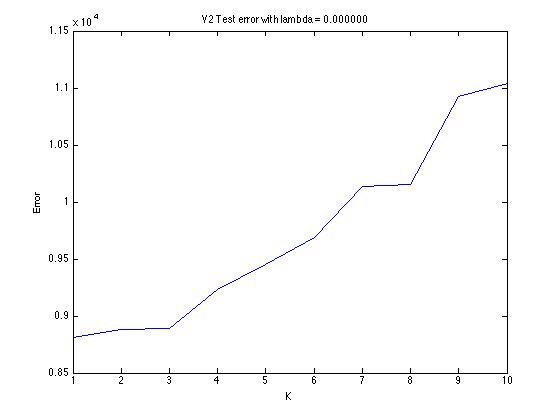
\includegraphics[scale=0.5]{TestErrorLambda0-V2.jpg}
\caption{ $E_{te}$ as of K with $\lambda=0.0$:}
\label{}
\end{figure}

\begin{figure}[H]
\centering
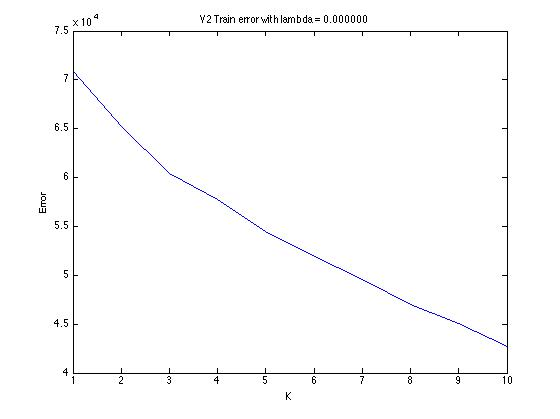
\includegraphics[scale=0.5]{TrainErrorLambda0-V2.jpg}
\caption{ $E_{tr}$ as of K with $\lambda=0.0$:}
\label{}
\end{figure}

\begin{figure}[H]
\centering
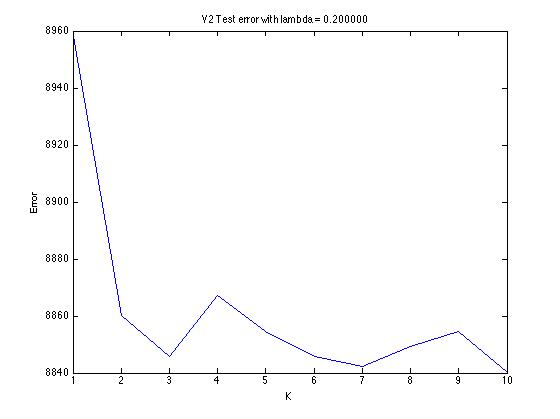
\includegraphics[scale=0.5]{TestErrorLambda02-V2.jpg}
\caption{ $E_{te}$ as of K with $\lambda=0.2$:}
\label{}
\end{figure}

\begin{figure}[H]
\centering
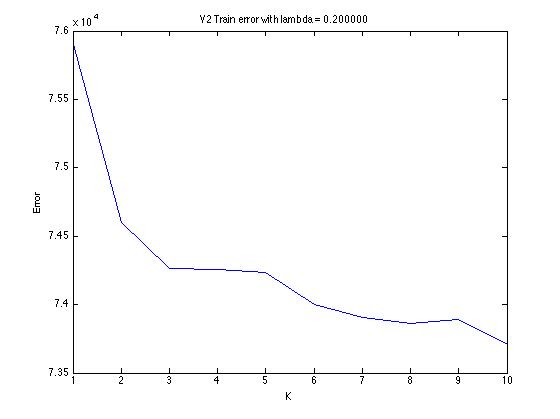
\includegraphics[scale=0.5]{TrainErrorLambda02-V2.jpg}
\caption{ $E_{tr}$ as of K with $\lambda=0.2$:}
\label{}
\end{figure}


\section{Question 2 -- PageRank Computation}
\subsection{(a)}
$r - r^{(k)} = \beta Mr - \beta Mr^{(k-1)} \\
=\beta M(r - r^{(k-1)}) \\
=\beta^2M^2(r - r^{(k-2)}) \\
=... \\
=\beta^kM^k(r - r^{(0)})$ \\
$M$ is stochastic, $\|M^kr\|_1 <= 1, \|M^kr^{(0)}\|_1 <= 1$ \\
So $\|r - r^{(k)}\|_1 <= \|\beta^k M^kr\|_1 + \|\beta^k M^kr^{(0)}\|_1 <= 2\beta^k$

\subsection{(b)}
Let $I$ be the number of iterations. \\
$\|r - r^{(I)}\|_1<= 2\beta^I <= \delta$\\
$I >= \log_\beta (\delta/2) = \frac{\log (2/\delta)}{\log (1/\beta)}$
We need iterate through every edge one time for each iteration. So total running time is: \\
$Im = m \frac{\log (2/\delta)}{\log (1/\beta)} = O({\frac{m}{\log (1/\beta)}})$



\subsection{(c)}
Let $c_j$ be the total number of visits at node j, Then $r_j = c_j\frac{1-\beta}{nR}$\\
Based on the algorithm, we have: $E[c_j] = \sum_{i->j} \beta \frac{E[c_i]}{deg(i)} + R$ \\
So, $E[\tilde{r_j}] = E[c_j]\frac{1-\beta}{nR} = \sum_{i->j} \beta \frac{E[c_i]\frac{1-\beta}{nR}}{deg(i)} + \frac{1-\beta}{n} \\
= \sum_{i->j} \beta \frac{E[c_i\frac{1-\beta}{nR}]}{deg(i)} + \frac{1-\beta}{n} \\
= \sum_{i->j} \beta \frac{E[\tilde{r_i}]}{deg(i)} + \frac{1-\beta}{n}$ \\
Which can be re-written as: $E[\tilde{r_j}] = \frac{1-\beta}{n}\textbf{1}^T + \beta ME[\tilde{r_j}]$ \\
We also have: $r_j = \frac{1-\beta}{n}\textbf{1}^T + \beta Mr_j$ \\
So $E[\tilde{r_j}] = r_j$


\subsection{(d)}
Expected run time of one random walker $E[w] = \sum_{i=1}^{\infty}i(1-\beta)\beta^{i-1}=\frac{1}{1-\beta}$\\
Expected running time of MC algorithm is: $E[w]\cdot nR = \frac{nR}{1-\beta}$
\end{document}